%!TEX root = ../Thesis.tex
%Chapter 2

\chapter{$S$-matrix pole symmetries for non-Hermitian scattering Hamiltonians}
\label{Chapter2}
\lhead{Chapter 2. \emph{$S$-matrix pole symmetries for non-Hermitian scattering \\Hamiltonians}}

Non-Hermitian Hamiltonians may have in general complex eigenvalues. However, in 1998 Carl M. Bender showed that non-Hermitian potentials having PT-symmetry can have a completely real spectra \cite{Bender1998}. Later, in a series of works published in 2002, Ali Mostafazadeh generalized this finding \cite{Mostafazadeh2002,Mostafazadeh2002a,Mostafazadeh2002b}. A Hamiltonian with a discrete spectrum that satisifies \eqref{eq:chapter1_symmetry}, for a Hermitian and antilinear operator $A_{antilinear}$; or \eqref{eq:chapter1_pseudoSymmetry} for a Hermitian and linear operator $A_{linear}$, will have eigenvalues that are real or come in complex-conjugate pairs \cite{Mostafazadeh2002,Mostafazadeh2002a,Mostafazadeh2002b}. An aspect uncovered in refs. \cite{Mostafazadeh2002,Mostafazadeh2002a,Mostafazadeh2002b} is that, under the same conditions, the complex poles of the scattering matrix can also come in complex conjugate pairs.

This chapter aims at extending the results in chapter \ref{Chapter1} and refs. \cite{Mostafazadeh2002,Mostafazadeh2002a,Mostafazadeh2002b} in several directions:

i) I will provide an alternative characterization of the 8 symmetries formed by the elements of the Klein 4-group and the relations \eqref{eq:chapter1_symmetry}, \eqref{eq:chapter1_pseudoSymmetry} in terms of the invariance of $H$ with respect to the action of superoperators.

ii) Moreover,
four of these eight symmetries imply the same
type of pole structure of $S$-matrix eigenvalues in the complex momentum plane that was found for PT symmetry \cite{Muga2004},
namely, zero-pole correspondence at complex-conjugate points, and poles on the imaginary axis or forming symmetrical pairs with respect to the imaginary
axis. This configuration with poles located on the imaginary  axis or as symmetrical pairs has some important consequences. In particular, it provides stability of the real energy eigenvalues with respect to parameter variations of the potential. While a simple pole on the imaginary axis can move along that axis when a parameter is changed, it cannot move off this axis (since this would violate the pole-pair symmetry) or bifurcate. The formation of pole pairs occurs near special  parameter values for which two poles on the imaginary axis collide. When the poles are mapped to the energy complex plane $E = p^2/2m$, they have the same symmetry structure of complex conjugate pairs as the discrete eigenvalues of an $A$-pseudohermitian Hamiltonian, which expands the results of refs. \cite{Mostafazadeh2002,Mostafazadeh2002a,Mostafazadeh2002b}.

The remainder of the chapter is organized as follows. In section \ref{sec:chapter2_super}, I characterize the symmetry operations defined in chapter \ref{Chapter1} as the invariance of the Hamiltonian with respect to the action of eight linear or antilinear superoperators. In section \ref{sec:chapter2_SPoles}, I discuss the physical consequences of the symmetries in the pole structure of the scattering matrix eigenvalues. Four symmetries are shown to lead to complex poles corresponding to real energies or conjugate (energy) pairs. This result generalizes what was found in refs. \cite{Mostafazadeh2002,Mostafazadeh2002a,Mostafazadeh2002b}. In section \ref{sec:chapter2_separablePotentials}, I exemplify the general results with separable potentials exhibiting parity-pseudohermiticity and time-reversal symmetry. These are the two non-trivial symmetries of the four which have complex-conjugate pairs of eigenvalues (in the sense that the other two, hermiticity and PT-symmetry, are already well discussed). In section \ref{sec:chapter2_Discussion}, I discuss and summarize the results.
%
\begin{landscape}
  \begin{table}
    \centering
    \caption{Symmetries of the Hamiltonian with respect to the commutativity or pseudohermiticity of $H$ with the elements of $\mathbf{K}_4$ (column 2) in terms of the action of superoperators $\mathcal{L}$ on the potential $V$ in coordinate (Column 4) or momentum (Column 6) representation. This table follows the same code convention with roman numbers for the symmetries as chapter \ref{Chapter1} and can be seen as an extension of table \ref{tab:chapter1_SymmetriesTable} incorporating the superoperator formalism
    \vspace*{.2cm}
    \label{tab:chapter2_Symmetries}}
    \scalebox{1}{
    \begin{tabular}{ccccccccccc}
      \hline
      \hline\\
      (1)&(2)&(3)&(4)&(5)&(6)&(7)&(8)&(9)&(10)&(11)
      \\
      Code & Symmetry&  $\la x|V|y\ra$ & ${\cal{L}}$(coord)& $\la p|V|p'\ra$ & ${\cal L}$(momentum) &$\la p|S|p'\ra$ & $T^l$ & $T^r$ & $R^l$& $R^r$
      \\
      \hline
      I & $1H=H1$ &   $\la x|V|y\ra$ & ${ 1}$ &$\la p|V|p'\ra$ &${ 1}$& $\la p|S|p'\ra$ & $T^l$ & $T^r$ & $R^l$ & $R^r$
      \\
      II & $1H=H^\dagger 1$ &  $\la y|V|x\ra^*$ & ${\cal TC}$& $\la p'|V|p\ra^*$ &${\cal T'C'}$&$\la p|\widehat{S}|p'\ra$ & $\widehat{T}^l$& $\widehat{T}^r$ & $\widehat{R}^l$ & $\widehat{R}^r$
      \\
      III & $\Pi H=H\Pi$ &  $\la -x|V|-y\ra$ &${\cal I}$&  $\la -p|V|-p'\ra$ &${\cal I'}$&$\la -p|S|-p'\ra$ & $T^r$ & $T^l$ & $R^r$ & $R^l$
      \\
      IV & $\Pi H=H^\dagger \Pi$ &  $\la -y|V|-x\ra^*$ &${\cal CTI}$& $\la -p'|V|-p\ra^*$ &${\cal C'T'I'}$& $\la -p|\widehat{S}|-p'\ra$ & $\widehat{T}^r$ & $\widehat{T}^l$ & $\widehat{R}^r$ & $\widehat{R}^l$
      \\
      V & $\Theta H=H\Theta$ &  $\la x|V|y\ra^*$&${\cal C}$& $\la -p|V|-p'\ra^*$ &${\cal I'C'}$& $\la -p'|\widehat{S}|-p\ra$ & $\widehat{T}^r$ & $\widehat{T}^l$ & $\widehat{R}^l$& $\widehat{R}^r$
      \\
      VI & $\Theta H=H^\dagger\Theta$ &  $\la y|V|x\ra$&${\cal T}$& $\la -p'|V|-p\ra$ &${\cal I'T'}$& $\la -p'|S|-p\ra$ & $T^r$& $T^l$ & $R^l$& $R^r$
      \\
      VII & $\Theta\Pi H=H\Theta \Pi$ &  $\la -x|V|-y\ra^*$ &${\cal IC}$& $\la p|V|p'\ra^*$ &${\cal C'}$& $\la p'|\widehat{S}|p\ra$ &$\widehat{T}^l$& $\widehat{T}^r$ & $\widehat{R}^r$& $\widehat{R}^l$
      \\
      VIII& $\Theta\Pi H=H^\dagger \Theta \Pi$ &  $\la -y|V|-x\ra$ &${\cal IT}$& $\la p'|V|p\ra$ &${\cal T'}$& $\la p'|S|p\ra$ & $T^l$ & $T^r$ & $R^r$ & $R^l$
      \\
      \hline
      \hline
    \end{tabular}
    }
  \end{table}
\end{landscape}
% -------------------------------------------------------------------------------------------------


\section{Superoperator formalism\label{sec:chapter2_super}}

The eight symmetries discussed in chapter \ref{Chapter1}, which are listed again in Table \ref{tab:chapter2_Symmetries} may also be regarded as the invariance of the Hamiltonian with respect to
transformations represented by superoperators ${\cal L}$ \cite{Simon2018} defined by
%
\begin{equation}
	\mathcal{L}(H)=
	\begin{cases}
		A^\dagger H A &  \text{I, III,V,VII} \\
		A^\dagger H^\dagger A &\text{II, IV, VI, VIII}
		\end{cases}.
\end{equation}
%
This definition of the superoperator action is independent of the representation we use, but its realization in coordinates or momenta representation in terms of the operations of complex conjugation $\mathcal{C}$, transposition $\mathcal{T}$, and inversion $\mathcal{I}$ (sign reversal of momentum or position), is different. In coordinate representation, these superoperators take the following forms (see column 3 in Table \ref{tab:chapter2_Symmetries}),
%
\begin{align}
	1 H&=\int\!\!\int |x\ra \la x|H|y\ra\la y| dx dy,
	\nonumber\\
	{\cal T} (H) &=\int\!\!\int |x\ra \la y|H|x\ra\la y| dx dy,
	\nonumber\\
	{\cal C} (H)&=\int\!\!\int |x\ra \la x|H|y\ra^*\la y| dx dy,
	\nonumber\\
	{\cal I} (H)&=\int\!\!\int |x\ra \la -x|H|-y\ra\la y| dx dy,
	\label{eq:chapter2_superoperatorsPosition}
\end{align}
%
while in momentum representation, these superoperators are
%
\begin{align}
	1 H&=\int\!\!\int |p\ra \la p|H|q\ra\la q| dp dq,
	\nonumber\\
	{\cal T}' (H) &=\int\!\!\int |p\ra \la q|H|p\ra\la q| dp dq,
	\nonumber\\
	{\cal C}' (H)&=\int\!\!\int |p\ra \la p|H|q\ra^*\la q| dp dq,
	\nonumber\\
	{\cal I}' (H)&=\int\!\!\int |p\ra \la -p|H|-q\ra\la q| dp dq.
	\label{eq:chapter2_superoperatorsMomentum}
\end{align}
%
Adopting the trace inner product for linear operators $F$ and $G$
%
\begin{equation}
  \langle\langle F|G\rangle\rangle={\rm{tr}} (F^\dagger G)
  \label{eq:chapter1_innerProduct}
\end{equation}
%
we can show that all superoperators (also the primmed ones) and their products ${\cal L}$ are either unitary (for ${\cal L}=1,{\cal T},{\cal I},{\cal TI}$), or antiunitary (for ${\cal L}={\cal C}, {\cal CT},{\cal CI},{\cal CTI}$), with respect to the inner product as defined by
%
\begin{eqnarray}
	\langle\langle {\cal L}F| {\cal L}G\rangle\rangle&=& \langle\langle F| G\rangle\rangle\;\;\;  ({\cal L}\; {\rm unitary}),
	\\
	\langle\langle {\cal L}F| {\cal L} G\rangle\rangle&=& \langle\langle  F| G\rangle\rangle^*\;\;\;  ({\cal L}\; {\rm antiunitary}).
\end{eqnarray}
%
They all satisfy ${\cal L}{\cal L}^\dagger={\cal L}^\dagger {\cal L}=1$
where the adjoints are defined differently for linear or antilinear superoperators,
\begin{eqnarray}
	\langle\langle F| {\cal L}^\dagger G\rangle\rangle&=& \langle\langle {\cal L} F| G\rangle\rangle\;\;\;  ({\cal L}\; {\rm unitary}),
	\\
	\langle\langle F| {\cal L}^\dagger G\rangle\rangle&=& \langle\langle {\cal L} F| G\rangle\rangle^*\;  ({\cal L}\; {\rm antiunitary}).
\end{eqnarray}
%
Moreover the eight superoperators  satisfy ${\cal L}^\dagger={\cal L}$.

The set $\{1, \cal{I,T,C,CT,TI,IC,CTI}\}$ (and the primmed ones) forms the elementary Abelian group $E8$ \cite{Rose2009}. This is a homocyclic group, namely, the direct product of isomorphic
cyclic groups of order 2 with generators $\cal{C,T,I}$. Only for the subgroup $\{1, \cal{I,CT,CTI}\}$ the superoperators have the same representation-independent form in terms of complex conjugation, transposition, and inversion in momentum and position bases.

A direct application of the superoperator framework is the generalization of Wigner's
formulation of symmetries \cite{Wigner1959}. He associated symmetry transformations to unitary or antiunitary operators preserving the (Hilbert space) inner product, namely the ``transition probabilities'' $|\expval{A\psi,A\phi}|^2=|\expval{\psi,\phi}|^2$.
For general states described by density operators $\rho_1,\rho_2$, transition probabilities are computed as $\la\la \rho_1|\rho_2\ra\ra$
and the transformations described by the unitary or antiunitary superoperators preserve the
transition probability. Hamiltonian symmetries are, within the conventional Wigner scheme, the  symmetry transformations that leave the Hamiltonian invariant ($A^\dagger H A=H$, so that $A$ and $H$ commute). Here the Hamiltonian symmetry is more broadly defined  as
the invariance ${\cal L}H=H$, which includes transformations  beyond the conventional scheme.

\section{S-matrix pole structure}
\label{sec:chapter2_SPoles}
%
In refs. \cite{Mostafazadeh2002,Mostafazadeh2002a,Mostafazadeh2002b}, Mostafazadeh derived the sufficient and necessary conditions of diagonalizable Hamiltonians with a discrete spectrum for having a spectrum made of real eigenvalues and complex-conjugate pairs of eigenvalues. The condition was that the Hamiltonian had to be $A-$pseudohermitian with respect to a Hermitian linear operator $A$ or commute with a Hermitian antilinear operator $B$. In fact, the two conditions are equivalent \cite{Mostafazadeh2002b}: if a Hamiltonian is $A$-pseudohermitian one can find a Hermitian antilinear $B$ that commutes with $H$ and viceversa. In this section I generalize the results in \cite{Mostafazadeh2002,Mostafazadeh2002a,Mostafazadeh2002b} to scattering Hamiltonians. I show, for the symmetry operators in the Klein 4-group, that the poles of the $S-$matrix have the same structure as the eigenvalues of the discrete spectrum, as described in \cite{Mostafazadeh2002,Mostafazadeh2002a,Mostafazadeh2002b}, when the Hamiltonian satisfies symmetries V and VII of table \ref{tab:chapter2_Symmetries}, \textit{i.e.}, eq. \eqref{eq:chapter1_symmetry} for $A$ antiunitary ($A = \Theta,\Pi\Theta$), or symmetries II and IV of table \ref{tab:chapter2_Symmetries}, \textit{i.e.}, eq. \eqref{eq:chapter1_pseudoSymmetry} for A unitary ($A = 1,\Pi$).


In section \ref{sec:chapter1_ScattFormalism} we introduced the scattering matrix ($S$-matrix) formalism, which was used to derive the results of chapter \ref{Chapter1} regarding the scattering coefficients. It was possible to decompose the $S$-matrix into the on-the-energy-shell matrices $\sf{S}$ for real and positive momentum in terms of transmission and reflection amplitudes for right
and left incidence, see eq. \eqref{eq:chapter1_onShellMatrix}. The $\sf{S}$ matrix contains the scattering amplitudes for incoming wave packets with well defined momentum being scattered into states with the same kinetic energy and reflected and transmitted components. The on-shell scattering matrix $\mathsf{S}$ allowed us to obtain the generalized unitary relations \eqref{eq:chapter1_SMatrixUnitarityGeneralized} in terms of the scattering amplitudes \eqref{eq:chapter1_unitarityCoefficients}. For negative $p$ the matrix elements of $\mathsf{S}$ give the amplitudes of scattering states with a pure outgoing plane wave towards the right or the left. Moreover we assume, as it is customary, that the amplitudes may be continued analytically beyond the real axis. The existence of a continuation on the complex plane domain depends on decay properties of the potentials and may
be checked for each potential.
The analytical continuation is indeed possible for the model potentials of the following section.

We will look for the poles of the $S$-matrix in the eigenvalues of its on-shell decomposition $\mathsf{S}$. The eigenvalues of $\sf{S}$ can be calculated from the transmission and reflection amplitudes as
%
\begin{equation}
	S_j=\frac{(T^l+T^r)+(-1)^j[(T^l-T^r)^2+4R^lR^r]^{1/2}}{2}
	\label{eq:chapter2_SEigenvalues}
\end{equation}
%
for $j=1,2$, and of course there is a similar expression for $\widehat{S}_j$ (The scattering matrix for the adjoint Hamiltonian) with hatted amplitudes.
In general they satisfy the relations \cite{Muga2004},
%
\begin{equation}\label{eq:chapter2_pam1}
	S_j(p)=\widehat{S}_j^*(-p^*)\,,
\end{equation}
%
and
%
\begin{equation}\label{eq:chapter2_pam2}
	\widehat{S}_j^*(p^*)S_j(p)=1\,.
\end{equation}
%
Combining eqs. (\ref{eq:chapter2_pam1}) and (\ref{eq:chapter2_pam2}) gives
%
\begin{equation}\label{eq:chapter2_pam3}
	S_j(p)=S^{-1}_j(-p)\,.
\end{equation}
%
Equation \eqref{eq:chapter2_pam3} is remarkable since it reveals the presence of a pole (zero) at $-p$ if there is a zero (pole) at $p$.
%
If the following relations are fulfilled,
%
\begin{eqnarray}
	T^{r,l}(p)&=&\widehat{T}^{r,l}(p)\; {\rm or}\; T^{r,l}(p)=\widehat{T}^{l,r}(p),
	\label{ts}
	\\
	R^{r,l}(p)&=&\widehat{R}^{r,l}(p)\; {\rm or}\; R^{r,l}(p)=\widehat{R}^{l,r}(p),
	\label{rs}
\end{eqnarray}
%
then
%
\begin{equation}
	S_j(p)=\widehat{S}_j(p),
\end{equation}
%
which together with eq. \eqref{eq:chapter2_pam1} gives
%
\begin{equation}
	S_j(p)=S_j^*(-p^*).
	\label{eq:chapter2_PoleSymmetry}
\end{equation}
%}
In plain language, eq. \eqref{eq:chapter2_PoleSymmetry} tells that if eqs. (\ref{ts}) and (\ref{rs}) are satisfied,  the poles and zeros of $S_j$ must be symmetrically distributed with respect to the imaginary axis of the momentum complex plane. Combined with eq. (\ref{eq:chapter2_pam3})
this also means that each pole has a symmetrical zero with respect to the real axis. This symmetrical distribution of poles and zeros is the same as in the Hermitian case (see fig. \ref{fig:DiagramPoles}),
%end red
the only difference being the possibility
of finding pairs of symmetrical poles in the upper complex plane when $H\neq H^\dagger$. They represent normalizable ``bound states
with complex energies''. When they  are not present, the discrete spectrum becomes purely real.

According to Table \ref{tab:chapter2_Symmetries},  eqs. (\ref{ts}) and (\ref{rs}) are fulfilled
for symmetries  II (hermiticity), VII (PT-symmetry), IV (parity pseudohermiticity),
and V (time-reversal invariance). Thus, Hamiltonians having these symmetries have their $S-$matrix poles symmetrically distributed about the imaginary axis. For local potentials the last two symmetries coalesce with the first two well-known
cases \cite{Ruschhaupt2017}, namely,
IV becomes equivalent to PT-symmetry, and V becomes equivalent to hermiticity. For non-local potentials, though, these symmetries
correspond to genuinely distinct properties. In the following section we shall demonstrate this fact with potentials that are
either purely parity-pseudohermitian (and not PT-symmetrical), or time-reversal invariant but not Hermitian.
%


\begin{figure}[h]
  \centering
  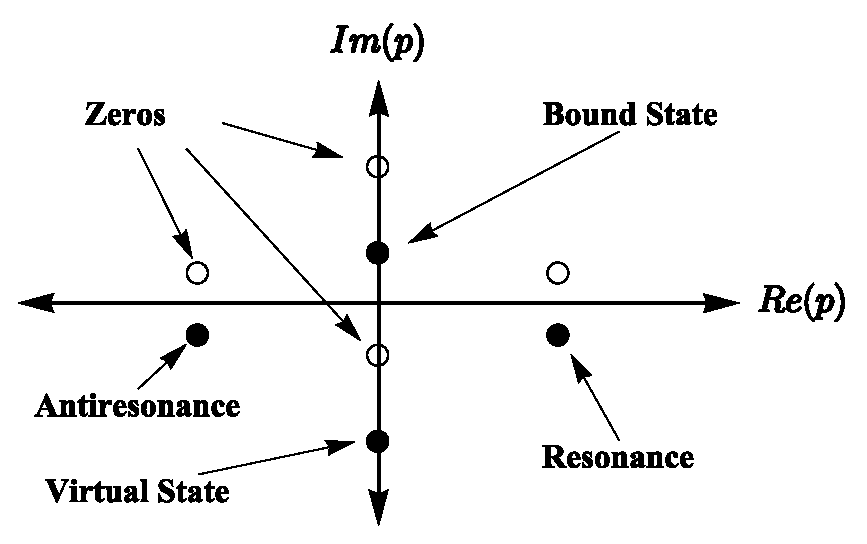
\includegraphics[width=0.5\linewidth]{Figures/DiagramPoles.eps}
  \caption{Example of configuration of poles (filled circles) and zeros (empty circles) of the $S$-matrix eigenvalues in the complex momentum plane for Hermitian Hamiltonians.  Poles in the upper half plane ($\operatorname{Im}(p) > 0$) correspond to bound eigenstates of the Hamiltonian, i.e. localized states with negative energy. Poles in the lower half plane correspond to  virtual states ($\operatorname{Re}(p) = 0$), resonances ($\operatorname{Re}(p) > 0$) and antiresonances ($\operatorname{Re}(p)<0$). The singularities with negative imaginary part correspond to states that do not belong to the Hilbert space since they are not normalizable. However, they can produce observable effects in the scattering amplitudes, in particular when they approach the real axis. The pole structure of symmetries IV, V, and VII, see Table \ref{tab:chapter2_Symmetries},
  is similar, but pole pairs are also possible in the upper half-plane.}
  \label{fig:DiagramPoles}
\end{figure}

\section{Separable Potentials}
\label{sec:chapter2_separablePotentials}
%
%
In order to illustrate and test the theoretical concepts that we have discussed, in particular the
symmetrical configuration of poles with respect to the imaginary axis in the complex momentum plane for certain Hamiltonian symmetries, we will use some solvable toy models consisting on rank-one separable potentials.
Separable potentials are quite useful models as a solvable approximation to realistic ones, in particular in nuclear, atomic, and molecular physics \cite{Popov2019}.
Often they lead to explicit expressions
for wave functions or scattering amplitudes, so they are used to test concepts and new methods.
They are also instrumental in learning about different dynamical phenomena (for example transient effects, short-time and long-time behavior, or anomalous decay laws)  and their relation to complex-plane singularities
\cite{Muga1990,Muga1996,Muga1996a,Muga1998}. Their simplest version takes the form
$|\chi\ra V_0\la\chi|$ for some  $\chi$.   In particular, with a complex $V_0$,
they have been used to examine anomalous (negative) time delays caused by  crossing of zeroes of the $S$-matrix eigenvalues or $S$-matrix elements across the momentum real axis \cite{Muga1998a}.

In this work we consider the simple structure
$V=V_0 \ketbra{\phi}{\chi}$, with $V_0$ (potential strength) real, and conveniently chosen normalised states $\ket{\phi}$, $\ket{\chi}$.
The aim of this section is to demonstrate the formal results of the previous section without attempting to simulate any specific systems, but we note that separable, non-Hermitian potentials are instrumental to model nuclear reactions, in particular  by increasing the rank (number of separable terms) \cite{Hlophe2017}.
Separable non-Hermitian potentials also provide solvable approximations to non-local non-Hermitian potentials that arise naturally in quantum optics to describe the interaction of a ground state atom with a laser beam \cite{Ruschhaupt2004a}.

I proceed to look for the poles of the ${\sf S}$ matrix in the following way. Since the scattering amplitudes in ${\sf S}$ are simply related to matrix elements of $T_{op}(z)$ (eq. \eqref{eq:chapter1_transitionOperator_definition}) in momentum representation, see eq. \eqref{eq:chapter1_amplitudesFromTOperator}, the singularities in the scattering amplitudes and the eigenvalues of ${\sf S}$ will come from the singularities of $T_{op}(z)$ \cite{Muga1996}. For a separable potential, the transition operator $T_{op}$ can be written (see Appendix \ref{Appendix:SeparablePotentials_TransitionOperator}) as
%
\begin{equation}
	T_{op}=\frac{V_{0}}{1-V_{0} Q_{0}(E)} \ketbra{\phi}{\chi},
  \label{eq:chapter2_TransitionOperatorSeparablePotential}
\end{equation}
%
where $Q_{0}(E)=\bra{\chi}(E-H_0)^{-1}\ket{\phi}$ and $H_{0}=p^{2}/(2m)$. Therefore, the singularities (poles) of ${\sf S}$ are found by solving
%
\begin{eqnarray}
	Q_{0}(E)V_{0} = 1,
	\label{eq:chapter2_roots}
\end{eqnarray}
%
Once $Q_{0}(E)$  is calculated, the transmission and reflection amplitudes can be found from \eqref{eq:chapter1_amplitudesFromTOperator} using the momentum representation of $\ket{\phi}$ and $\ket{\chi}$ (see Appendix \ref{Appendix:SeparablePotentials_AmplitudesAndEigenvaluesofS}).

In the following subsections I will build a Hamiltonian with symmetry V (time reversal) and another one with symmetry IV (parity pseudohermicity) and illustrate the symmetries of the $\mathsf{S}$ matrix poles in momentum complex plane.
%
\subsection{Time-reversal symmetric potential}
%
%
\begin{figure}[h]
  \centering
	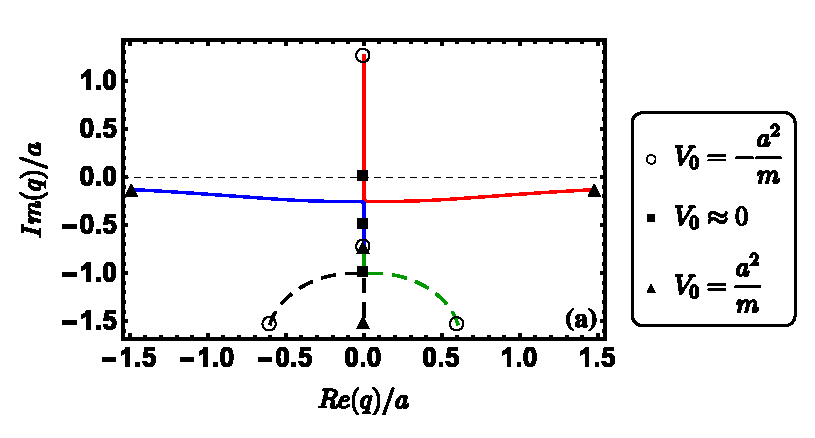
\includegraphics[width=0.75\linewidth]{Figures/VSymEigenvalsVaryingV0_Momentum.eps}
	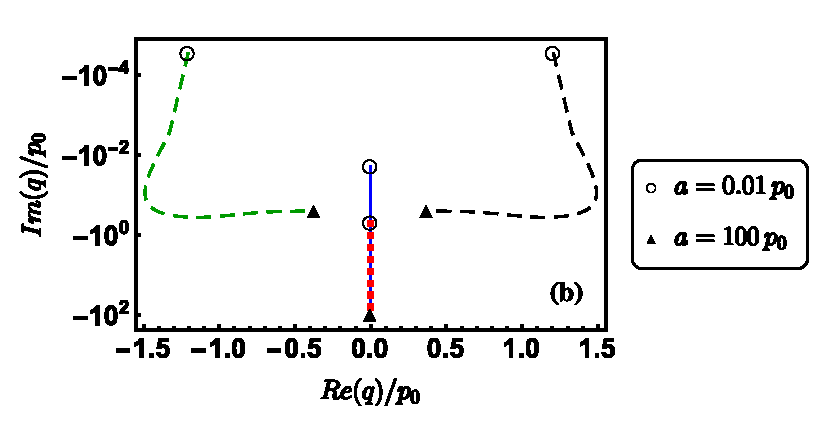
\includegraphics[width=0.75\linewidth]{Figures/VSymEigenvalsVaryingA_Momentum_Log.eps}
	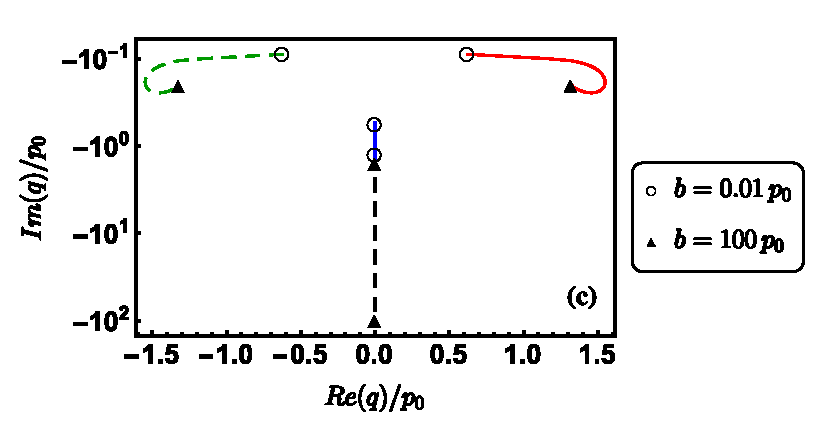
\includegraphics[width=0.75\linewidth]{Figures/VSymEigenvalsVaryingB_Momentum_Log.eps}
	\caption{ Poles and pole trajectories of time-reversal symmetric potential \eqref{TRpot} for (a) varying $V_0$ with $a=2 b$; (b) varying $a$ with $b=0.5\, p_0$, $V_0>0$; and (c) varying $b$ with $a=p_0$,
	$V_0>0$. At pole collisions we connect each of the incoming trajectories with a different emerging trajectory but the choice of outgoing branch  is arbitrary since the two colliding poles lose their identity.}
	\label{fig:VSymEigenvals}
\end{figure}

We start with an example of a separable potential which only satisfies symmetry V (apart from the trivial symmetry I). The normalised vector $\ket{\chi}$, is given in position and momentum representation as
%
\begin{eqnarray}
	\braket{x}{\chi}&=&\sqrt{\frac{a}{\hbar}} e^{-a \left| x \right|/\hbar},
	\nonumber \\
	\braket{p}{\chi}&=& \sqrt{\frac{2 a^3}{\pi}} \frac{1}{p^2+a^2}.
\end{eqnarray}
%
We choose $\ket{\phi}$ similarly as
%
\begin{eqnarray}
	\braket{x}{\phi}=&\sqrt{\frac{2ab}{\hbar (a+b)}} \begin{cases}
	e^{-b x/\hbar} &x>0,\\ e^{a x/\hbar}  &x<0,
	\end{cases}\nonumber \\
	\braket{p}{\phi}=& \sqrt{\frac{ab}{\pi (a+b)}}\frac{a+b}{(p+i a)(p-i b)}.
\end{eqnarray}
%
The real and positive parameters $\hbar/ a$ and $\hbar/ b$ determine the width of the potential functions in coordinate representation.
$b$ is chosen different from $a$ to introduce a right/left  asymmetry in $\braket{x}{\phi}$.
In coordinate representation the potential is given as
%
\begin{eqnarray}
	\la x|V|y\ra = V_{0} \sqrt{\frac{2 b a^2}{\hbar^2 (a+b)}} \begin{cases}
	e^{-(a \left| y \right|+b x)/\hbar} \, &x>0,\\ e^{a (x-\left| y \right|)/\hbar} \,  &x<0.
\end{cases} \label{TRpot}
\end{eqnarray}
%
%which can be seen in fig. \ref{fig:VSymPotentialPlot}.
Clearly the potential is always even in $y$ and in the limiting case where $a=b$, it is also even in $x$. For $a=b$, the potential will satisfy parity symmetry (III) and also PT symmetry (VII), without asymmetric transmission or reflection.
% so we ignore it hereafter.

We define first a complex momentum $q=\sqrt{2 m E}$ (for complex $E$) with positive imaginary part.
To calculate $Q_{0}(q)$ explicitly we use a closure relation in momentum representation, and
complex contour integration around the poles at $ia$, $q$ and $ib$.
The result is then analytically continued to the whole $q$-plane,
%
\begin{equation}
Q_{0}(q)/m = -\frac{i \sqrt{2b} \left[2 a (a+b)^2-q^2 (3 a+b)-i q (2 a+b) (3 a+b)\right]}{q (a+b)^{3/2} (a-i q)^2 (b-i q)},
\label{eq:chapter2_ResolvantVSymm}
\end{equation}
%
with which we may calculate the transmission and reflection amplitudes.
The four roots of eq. (\ref{eq:chapter2_roots}) are the core poles of ${\sf S}$.

Using $m$, $V_0$ and $\hbar$ we define the length and momentum scales $L_0 = \hbar/\sqrt{mV_0}$ and $p_0 = \sqrt{mV_0}$. In fig. \ref{fig:VSymEigenvals}(a), we can see the trajectory of the ${\sf S}$-matrix core poles (zeros
of $1-V_0Q_0(q))$ for varying $V_0$. Notice a bound state for $V_0<0$ and collisions of the eigenvalue pairs around $V_0 = 0$. In figs. \ref{fig:VSymEigenvals}(b) and \ref{fig:VSymEigenvals}(c), where $V_0$ is positive and $a$ or $b$ are varied,
there are two virtual states and one resonance/anti-resonance pair. In all cases the symmetry of the poles about the imaginary axis
% for fig. \ref{fig:VSymEigenvals},
which corresponds to real energies or complex-conjugate pairs of energies, is evident. For larger values of the $a$ or $b$ parameters
(not shown)
the pair collides so that all poles end up as virtual states.

Figure \ref{fig:VSymScattAmplitudes} depicts the associated transmission and reflection coefficients (square moduli of the amplitudes) as functions of the momentum $p$. $|R^l(p)|=|R^r(p)|$ for all $p$ due to symmetry V, see column (11) of table \ref{tab:chapter1_SymmetriesTable}. The coefficients can be greater than one in contrast to the Hermitian case.

%%%%%%%%%%%%%%%%%%%%%%%%%%%%%%%%%%%%%%%%%%
%Figure
%%%%%%%%%%%%%%%%%%%%%%%%%%%%%%%%%%%%%%%%%%
\begin{figure}
\begin{center}
	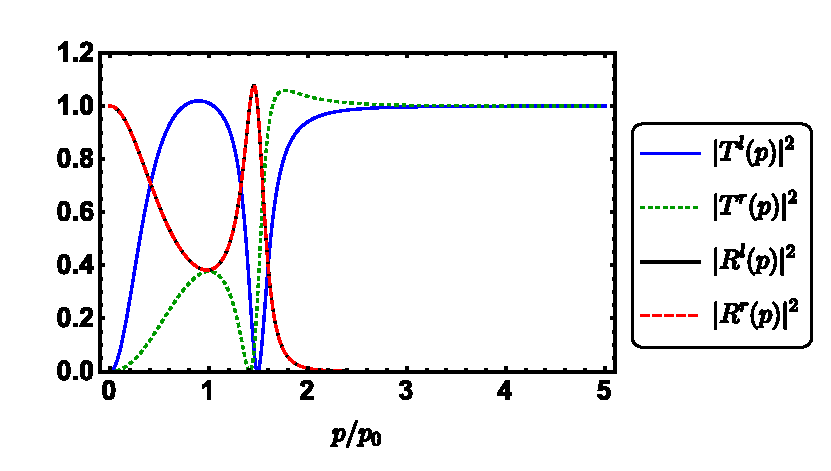
\includegraphics[width=0.75\linewidth]{Figures/VSymScattAmplitudes.eps}
\end{center}
\caption{Transmission and reflection coefficients of the time-reversal symmetric potential (symmetry V) \eqref{TRpot} with $a=p_0$, $b= 0.5\, p_0$ and $V_0>0$.}
\label{fig:VSymScattAmplitudes}
\end{figure}
%%%%%%%%%%%%%%%%%%%%%%%%%%%%%%%%%%%%%%%%%%

%
\subsection{Parity pseudohermitian potential}
%
%
As a second example we will consider  a separable potential which only fulfills symmetry IV. The normalised vector $\ket{\chi}$ in position and momentum representation is
%
\begin{eqnarray}
\braket{x}{\chi}=& \sqrt{\frac{a}{\hbar}} \begin{cases}
e^{-(a+ib)x/\hbar}  &x>0,\\ e^{a x/\hbar} &x<0,
\end{cases} \nonumber \\
\braket{p}{\chi}=&  \sqrt{\frac{a}{2\pi}} \frac{2 a+ i b}{(p+ia)(p+b-i a)},
\end{eqnarray}
%
where $a>0$ and $b$ is real.
We choose $\ket{\phi}$ as
%
\begin{eqnarray}
\braket{x}{\phi}=& \sqrt{\frac{a}{\hbar}} \begin{cases}
e^{-a x/\hbar} &x>0,\\ e^{(a+i b)x/\hbar} &x<0,
\end{cases} \nonumber \\
\braket{p}{\phi}=& \sqrt{\frac{a}{2\pi}} \frac{2 a+i b}{(p-ia)(p-b+i a)},
\end{eqnarray}
%
where $\hbar/a$ gives, as before, the width in coordinate representation. The potential functions in coordinate representation become asymmetrical
because of the  imaginary terms  $ib$ in  the exponent added only on  one side. This term leads to oscillations in real and imaginary parts. In momentum representation $b$ appears as a real shift in the position of one of the poles.
%
In coordinate representation the potential is
%
\begin{eqnarray}
\hspace*{-0.6cm}\la x|V|y\ra=  \frac{aV_{0}}{\hbar} \begin{cases}
e^{-\left[a (x+y) - i b y\right]/\hbar} \, ,&x>0,\,y>0\\
e^{a(y-x)/\hbar} \,  ,&x>0, \,y<0\\
e^{\left[a(x-y)+i b(x+y)\right]/\hbar} \,  ,&x<0,\,y>0\\
e^{\left[a(x+y)+i b x\right]/\hbar} \,  ,&x<0,\,y<0
\end{cases}.
\label{Ppot}
\end{eqnarray}
%
%see fig. \ref{fig:IVSymPotentialPlot}.
The case $b=0$ implies that the potential is real and hence satisfies time-reversal symmetry (V) with equal reflection amplitudes (as in the previous case), and also symmetry VIII.


\begin{figure}[h]
\centering
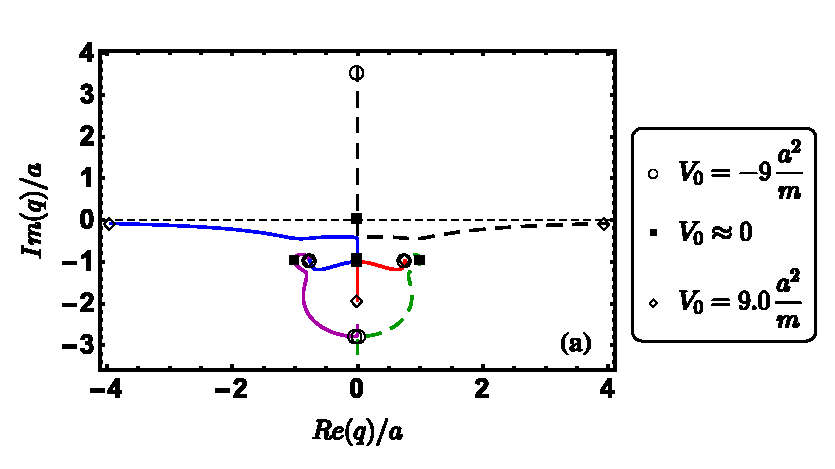
\includegraphics[width=0.75\linewidth]{Figures/IVSymEigenvalsVaryingV0new.eps}
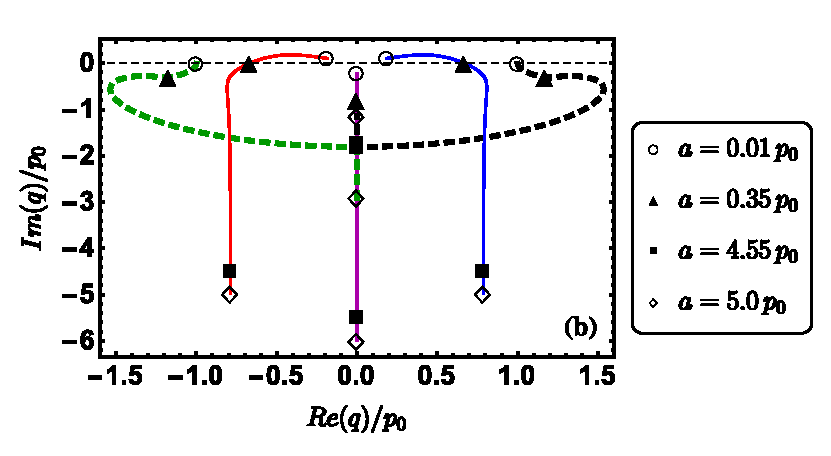
\includegraphics[width=0.75\linewidth]{Figures/IVSymEigenvalsVaryinganew.eps}
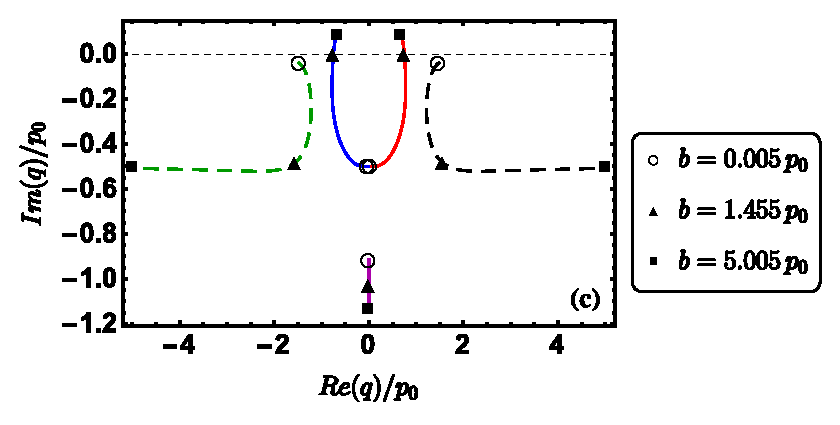
\includegraphics[width=0.75\linewidth]{Figures/IVSymEigenvalsVaryingbnew.eps}
\caption{ Poles and pole trajectories for the parity pseudohermitian potential \eqref{Ppot} (a) varying $V_0$ with $a=b$; (b) varying $a$ with $b=p_0$, $V_0>0$; (c) varying $b$ with $a=0.5\, p_0$, $V_0>0$.}
\label{fig:IVSymEigenvals}
\end{figure}



By calculating $Q_{0}$ again explicitly using complex contour integration around the poles at $-q$, $-b-i a$ and $b-i a$, we get that
%
\begin{equation}
Q_{0}(q)/m
=
\frac{8 a^2 q^3-4 a^2 q \left(10 a^2+b^2\right)-i a \left(4 a^2+b^2\right)^2+32 i a^3 q^2}{q \left(4 a^2+b^2\right) (a-i q)^2 \left[b^2+(a-i q)^2\right]}.
\nonumber\\
\end{equation}
%
Equation \eqref{eq:chapter2_roots} has five roots in this case constituting core poles of the $\mathsf{S}$-matrix elements.

Figure \ref{fig:IVSymEigenvals} depicts the trajectories of these poles for varying $a$, $b$ or $V_0$. As for the previous potential, the poles are symmetric with respect to the imaginary axis. In fig. \ref{fig:IVSymEigenvals}(a) there is a single bound state for $V_0<0$ while for positive values there are a resonance/antiresonance pair and a pair of virtual states. There are collisions of eigenvalues for values of $V_0$ close to 0. In fig. \ref{fig:IVSymEigenvals}(b)  two complex-conjugate (bound) eigenvalues cross the real axis and become a resonance/antiresonance pair. At the exact point where the eigenvalues are on the real axis, the scattering amplitudes diverge, however the eigenvalues of the $S$ matrix do not, since divergences of the left and right amplitudes cancel each other. For $a  \approx 4.55$ $p_0$ a resonance/antiresonance pair collides and becomes a pair of virtual states. In fig. \ref{fig:IVSymEigenvals}(c) another crossing of the real axis takes place, but in this case when decreasing $b$.

Figure \ref{fig:T_R_fig2} depicts the associated transmission and reflection coefficients as functions of the momentum $p$. The eigenvalues are not always equal since parity pseudohermicity does not imply any strict restriction to them \cite{Ruschhaupt2017}. For large  momenta, i.e. $p \gg \sqrt{2} p_0$, the potential is transparent giving $T^l,T^r \approx 1$. For $p\approx 1.5$ $p_0$ the right incidence transmission has a pronounced peak. Comparing with \ref{fig:IVSymEigenvals}(c), we notice that the values of the potential parameters and the momentum are close to the ones for which the real axis crossing takes place. Around $p = 0.6$ $p_0$ the potential acts as a $\mathcal{T}/\mathcal{R}$ device or one-way-barrier (see table \ref{tab:chapter1_DevicesDescription}).


\begin{figure}[t]
\begin{center}
  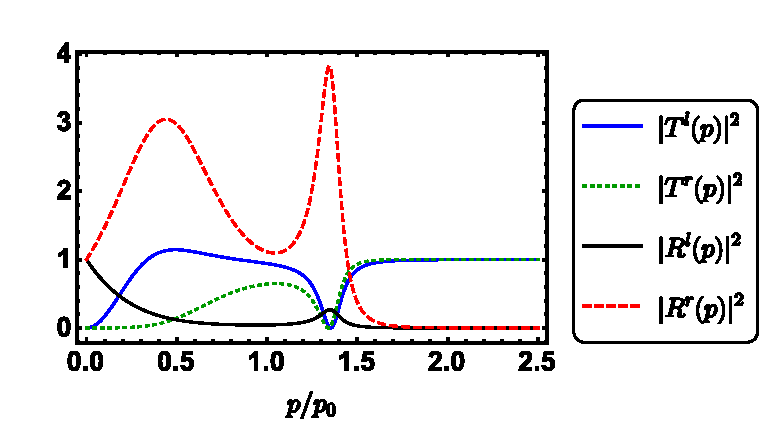
\includegraphics[width=0.75\linewidth]{Figures/IVSymTR.eps}
\end{center}
\caption{ Transmission and reflection coefficients for $a=b=0.5\, p_0$ and $V_0>0$.}
\label{fig:T_R_fig2}
\end{figure}


\section{Discussion}
\label{sec:chapter2_Discussion}

In this chapter I have studied some aspects of the scattering of a structureless particle in one dimension by
generally non-local and non-Hermitian potentials.

Conditions that were found for discrete Hamiltonians to imply conjugate pairs of discrete eigenenergies
(pseudohermiticity with respect to a linear operator or commutativity of $H$ with an antilinear operator \cite{Mostafazadeh2002,Mostafazadeh2002a,Mostafazadeh2002b}) can in fact be extended to scattering Hamiltonians in the continuum, implying symmetry relations not just for bound-state eigenvalues
but also for complex
poles of the $S$-matrix. Specifically the poles of $S$ matrix eigenvalues
are symmetrically located with respect to the imaginary axis, also in the lower momentum plane, so that resonances and antiresonance
energies are conjugate pairs as well.
In  terms of the eight possible Hamiltonian symmetries associated with Klein's group of $A$ operators (unity, parity, time reversal and PT)
and their commutation or pseudohermiticity with $H$,
the symmetrical disposition of the poles applies to four of them, which includes hermiticity and PT-symmetry. Potential models
and pole motions are provided for the
two other non trivial symmetries: time-reversal symmetry and parity pseudohermiticity.

% The study contributes to deepen our understanding of asymmetric scattering  (with different responses for left/right incidence) beyond the
% much studied  PT-symmetric potentials. This work opens interesting perspectives in AMO physics where much activity on asymmetric-scattering, mostly via optical devices,   is currently being carried out.
